\documentclass[a4paper]{article}

\usepackage{import}
\usepackage{xifthen}
\usepackage{pdfpages}
\usepackage{transparent}
\usepackage{xcolor}
\usepackage{tikz}
\usepackage{graphicx}
\graphicspath{ {figures/}, {/home/brandon/Documents/images/} }

\newcommand{\numpy}{{\tt numpy}}	% tt font for numpy
\newcommand{\incfig}[1]{%
	\def\svgwidth{\columnwidth}
	\import{./figures/}{#1.pdf_tex}
}
\pdfsuppresswarningpagegroup=1

\oddsidemargin -.25in
\evensidemargin -.25in
\textwidth 7in

\begin{document}
	\author{Brandon Thompson: 5517}
	\title{Lab 2: CEN4088.01 Due 9/26/2019}
	\maketitle

	\medskip
%	\vspace{4em}
	\begin{figure}[ht]
		\centering
		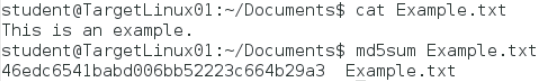
\includegraphics[width=0.8\textwidth]{1_2_7}
		\caption{MD5sum hash string for Example.txt.}
		\label{fig:1_2_7}
	\end{figure}

	\begin{figure}[ht]
		\centering
		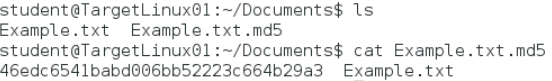
\includegraphics[width=0.8\textwidth]{1_2_11}
		\caption{Contents of Example.txt.md5 file.}
		\label{fig:1_2_11}
	\end{figure}

	\begin{figure}[ht]
		\centering
		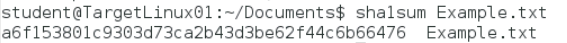
\includegraphics[width=0.8\textwidth]{1_2_15}
		\caption{SHA1sum hash string for Example.txt.}
		\label{fig:1_2_15}
	\end{figure}
	
	\begin{figure}[ht]
		\centering
		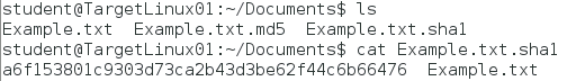
\includegraphics[width=0.8\textwidth]{1_2_19}
		\caption{Contents of Example.txt.sha1 file.}
		\label{fig:1_2_19}
	\end{figure}
	
	\begin{figure}[ht]
		\centering
		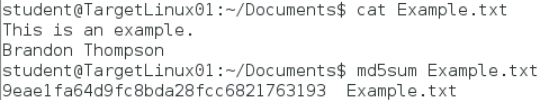
\includegraphics[width=0.8\textwidth]{1_3_4}
		\caption{Modified MD5sum hash string.}
		\label{fig:1_3_4}
	\end{figure}

	\begin{figure}[ht]
		\centering
		
\includegraphics[width=0.8\textwidth]{1_3_6}
		\caption{Modified SHA1 hash string.}
		\label{fig:1_3_6}
	\end{figure}

	\begin{figure}[ht]
		\centering
		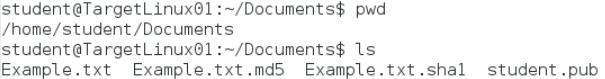
\includegraphics[width=0.8\textwidth]{1_4_13}
		\caption{Contents of /home/student/Documents directory.}
		\label{fig:1_4_13}
	\end{figure}

	\begin{figure}[ht]
		\centering
		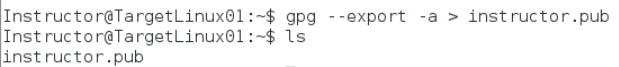
\includegraphics[width=0.8\textwidth]{1_4_21}
		\caption{Contents of /home/instructor directory.}
		\label{fig:1_4_21}
	\end{figure}

	\begin{figure}[ht]
		\centering
		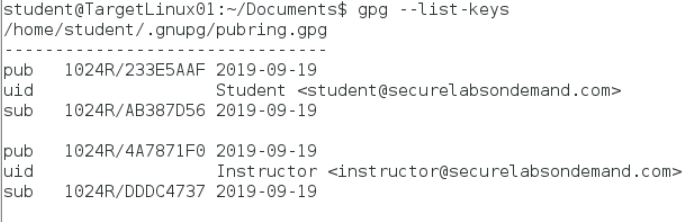
\includegraphics[width=0.8\textwidth]{1_5_6}
		\caption{List of strudent's public key ring.}
		\label{fig:1_5_6}
	\end{figure}

	\begin{figure}[ht]
		\centering
		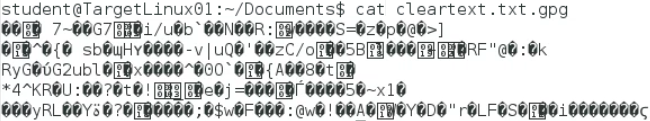
\includegraphics[width=0.8\textwidth]{1_6_8}
		\caption{Contents of encrypted cleartext.txt.gpg file.}
		\label{fig:1_6_8}
	\end{figure}

	\begin{figure}[ht]
		\centering
		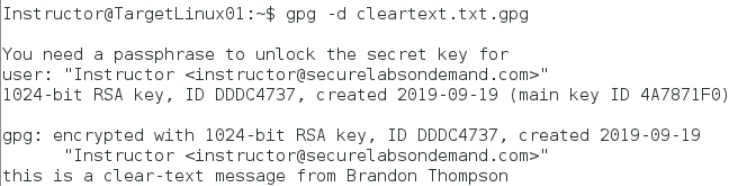
\includegraphics[width=0.8\textwidth]{1_6_19}
		\caption{Decrypted content of cleartext.txt.gpg file.}
		\label{fig:1_6_19}
	\end{figure}

	\begin{figure}[ht]
		\centering
		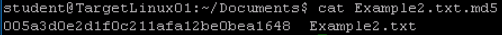
\includegraphics[width=0.8\textwidth]{2_2_6}
		\caption{Contents of Example.txt.md5 file.}
		\label{fig:2_2_6}
	\end{figure}
	\\
	\pagebreak
	\\
	\begin{figure}[ht]
		\centering
		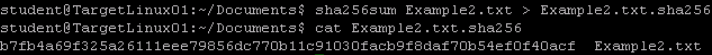
\includegraphics[width=0.8\textwidth]{2_2_13}
		\caption{Contents of Example2.txt.sha256 file.}
		\label{fig:2_2_13}
	\end{figure}

	\begin{figure}[ht]
		\centering
		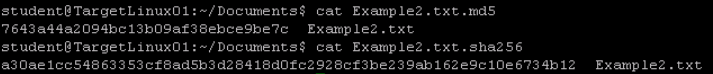
\includegraphics[width=0.8\textwidth]{2_3_7}
		\caption{Modified MD5sum and SHA-256 hash strings.}
		\label{fig:2_3_7}
	\end{figure}
	
	\begin{figure}[ht]
		\centering
		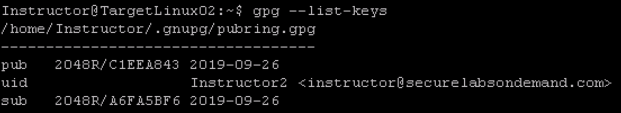
\includegraphics[width=0.8\textwidth]{2_4_17}
		\caption{Instructor's public key ring.}
		\label{fig:2_4_17}
	\end{figure}

	\begin{figure}[ht]
		\centering
		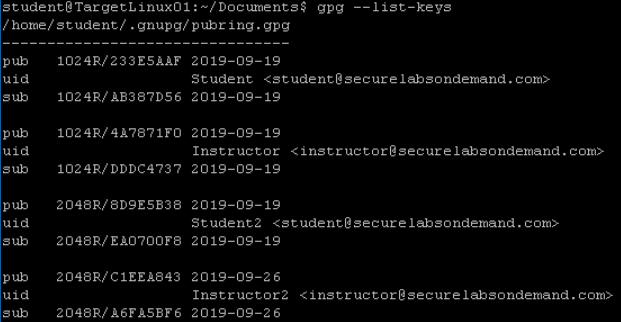
\includegraphics[width=0.8\textwidth]{2_5_12}
		\caption{Student's public key ring.}
		\label{fig:2_5_12}
	\end{figure}

	\begin{figure}[ht]
		\centering
		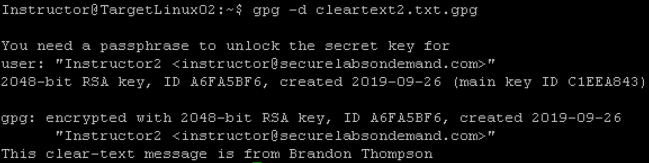
\includegraphics[width=0.8\textwidth]{2_6_19}
		\caption{Contents of decrypted cleartext2.txt.gpg.}
		\label{fig:2_6_19}
	\end{figure}
\end{document}
